\documentclass[12pt]{TDP005mall}
\usepackage{graphicx}
\usepackage{float}


\newcommand{\version}{Version 1.0}
\author{Elliot Johansson, \url{elljo130@student.liu.se}\\
  Lukas Freyland, \url{lukfr510@student.liu.se}\\
  Nadim Lakrouz, \url{nadla777@student.liu.se}}
\title{Kravspecifikation}
\date{2022-11-10}
\rhead{Elliot Johansson\\
Lukas Freyland\\
Nadim Lakrouz}



\begin{document}
\projectpage

\tableofcontents
\clearpage

\section{Revisionshistorik}
\begin{table}[!h]
\begin{tabularx}{\linewidth}{|l|X|l|}
\hline
Ver. & Revisionsbeskrivning & Datum \\\hline
1.0 & första utkast & 2022-11-10 \\\hline
\end{tabularx}
\end{table}


\section{Spelide}

Spelet utspelas i en 2D-värld där kameraperspektivet är uppifrån. Spelarens mål är att bekämpa flera vågor av attackerande fiender genom att använda kombinationer av magiska formler. Formlerna grundas av fyra element som sedan kombineras för att skapa olika typer av attacker. Fiender kommer röra sig emot spelaren och när de är tillräckligt nära kommer de explodera. Vid explosionen tar spelaren skada och fienden dör. Bland fienderna finns det olika typer och beroende på vilken typ tar den fienden mer skada av ett element än vad de andra fienderna skulle göra.\\
De magiska formlerna kommer spelaren kunna göra genom olika inmatningar. Spelaren kommer använda en eller två element för varje formel. Varje formel kostar ''Mana'' vilket begränsar vilka formler som spelaren kan använda beroende på hur mycket mana spelaren har. Spelaren får tillbaka ''Mana'' då ''Mana'' regenereras över tid. Det finns också en begränsning för att spelaren inte ska överanvända formler på en gång.
Spelaren kommer ha tillgång till att skapa olika magiska formler från början men kommer inte veta de olika kombinationerna för formeln och vad den gör. Så spelaren får testa sig fram och upptäcka alla formler själv. 


\subsection{Målgrupp}
Spelet är tänkt för unga personer som gillar action, strategi och att upptäcka nya saker.

\section{Spelupplevelse}
Spelaren får chansen att upptäcka själv vad hen kan göra för att bli bättre och klara sig längre. T.ex. då spelaren kommer lära sig flera nya magiska formler under varje spelomgång som hen kan använda för att besegra de inkommande fienderna. 

\clearpage

\subsection{Spelmekanik}
Spelaren kommer inte kunna flytta runt men kommer kunna använda sig av de olika grundformlerna för att attackera, läka eller skydda sig mot fiender.

\subsubsection{Knappar}
\begin{table}[H]
\begin{tabular}{|l|l|}
\hline
\textbf{Knapp} & \textbf{Element} \\ \hline
Q              & Vatten           \\ \hline
W              & Jord             \\ \hline
E              & Eld              \\ \hline
R              & Vind             \\ \hline
\end{tabular}\\
Tabell 1

\end{table}

\subsubsection{Grundläggande kombinationer}
\begin{table}[H]
\begin{tabular}{|l|l|}
\hline
\textbf{Knapp kombination} & \textbf{Magisk formel} \\ \hline
QQ                   & Vatten läknings formel \\ \hline
WW                   & Jord skölds formel     \\ \hline
EE                   & Eld klot formel        \\ \hline
RR                   & Virvelvinds formel     \\ \hline
\end{tabular}\\
Tabell 2

\end{table}

\subsubsection{Formler av kombinerade element}
\begin{table}[H]
\begin{tabular}{|l|l|}
\hline
\textbf{Knapp kombination} & \textbf{Magisk formel} \\ \hline
QW             & Lerpöl                 \\ \hline
QE             & Kokande vatten         \\ \hline
QR             & Tsunami                \\ \hline
WQ             & Jordskred              \\ \hline
WE             & Meteroitstorm          \\ \hline
WR             & Jordbävning            \\ \hline
EQ             & Ånga                   \\ \hline
EW             & Lava spray             \\ \hline
ER             & Stor eld ray           \\ \hline
RQ             & Hagelstrom             \\ \hline
RW             & Varmluft               \\ \hline
RE             & sandstrorm             \\ \hline
\end{tabular}\\
Tabell 3

\end{table}

\clearpage


\section{Regler}
\subsection{Spelplan}
En vertikal rektangel med fixerad storlek
\subsection{Spelare}
\begin{itemize}
\item Spelaren ser hela spelplanen
\item Spelaren står still
\item Spelaren kan kasta formler för att skada fiender och skydda sig själv.
\item Spelaren har ett visst antal liv
\item Spelaren har en viss mängd mana
\item När spelaren förlorat alla liv är spelet över
\end{itemize}
\subsection{poäng}
När spelaren dödar fiender får hen poäng.
\subsection{fiender}
Fienderna rör sig alltid mot spelaren och när den kolliderar med spelarens hitbox exploderar den och skadar spelaren med x antal skada. Fienderna har varierande livs poäng, hastighet och resistens mot element.
\section{visualisering}
\begin{center}
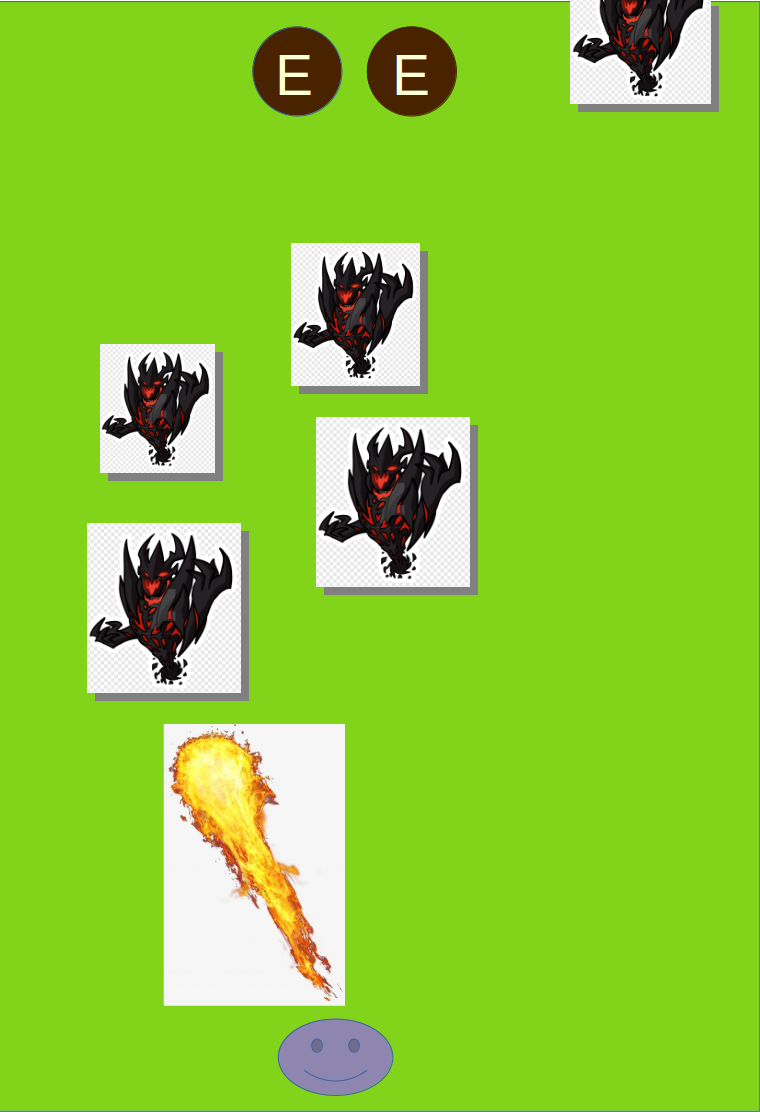
\includegraphics[scale=0.5]{spel.png}
\end{center}
\newpage

\section{Kravformulering}

\subsection{Ska-krav}
\begin{enumerate}
\item Det ska finnas ett spelarobjekt
\item Det ska finnas ett fiendeobjekt
\item Det ska gå att göra olika formler
\item Fyra grundformler ska finnas, se tabell 2.
\item QQ formeln ska göra att spelaren får tillbaka liv.
\item WW formeln ska skapa en köld som skyddar spelaren från skada.
\item EE formeln ska skjuta ett eldklot som skadar inkommande fiender.
\item RR formeln skapar en virvelvind som åker mot fienderna och skadar dem.
\item Spelaren ska kunna bestämma vilka formler som används med knappinmatning enligt tabell 2.
\item Spelaren ska ha ett visst antal liv.
\item Spelaren ska kunna ta skada av fiender.
\item Spelaren ska kunna göra skada på fiender med magiska formler
\item Fiender ska kunna göra skada när de kolliderar med spelarens hitbox.
\item Fiender ska alltid röra sig mot spelaren
\item Det ska finnas en startmeny
\item Spelet ska vara över när spelaren har slut på liv
\item Det ska finnas en mana mätare töms vid användning av formler
\item Mana ska regenerera över tid
\item Spelaren ser från ett 2D fågel perspektiv. 
\item Vi har gränsade väggar där fiender inte kan röra sig förbi.
\item Spelplanen är inte större än vad spelaren kan se.
\item Antal fiender och deras position kommer variera.
\item Fienders liv samt resistens mot attacker kommer variera

\clearpage

\subsection{Bör-krav}
\item Flera kombinationer av formler (se tabell 3) och flera element.
\item Poängsystem
\item Göra spelplan mer dynamisk så den intrigerar med spelarens handlingar.
\item Göra spelplanen och grafik i sidoperspektiv. 
\item Ha mer avancerade animationer.
\item Fiender bör ha resistens mot olika element.
\end{enumerate}


\section{Kravuppfyllelse}
\begin{enumerate}
    \item \textbf{Spelet ska simulera en värld som innehåller olika typer av objekt. Objekten ska ha olika beteenden och röra sig i världen och agera på olika sätt när de möter andra objekt.} \\ \emph{Krav: 1, 2, 3, 13, 12, 10.}
    
    \item \textbf{Det måste finnas minst tre olika typer av objekt och det ska finnas flera instanser av minst två av dessa. T.ex ett spelarobjekt och många instanser av två olika slags fiendeobjekt.} \\ \emph{Krav: 1, 2, 3}
    
    \item \textbf{Ett beteende som måste finnas med är att figurerna ska röra sig över skärmen. Rörelsen kan följa ett mönster och/eller vara slumpmässig. Minst ett objekt, utöver spelaren ska ha någon typ av rörelse.} \\ \emph{Krav: 13, 7, 8}
    
    \item \textbf{En figur ska styras av spelaren, antingen med tangentbordet eller med musen. Du kan även göra ett spel där man spelar två stycken genom att dela på tangentbordet (varje spelare använder olika tangenter). Då styr man var sin figur.} \\ \emph{Krav: 9}
    
    \item \textbf{Grafiken ska vara tvådimensionell.} \\ \emph{Krav: 18}
    
    \item \textbf{Världen (spelplanen) kan antas vara lika stor som fönstret (du kan göra en större spelplan med scrollning, men det blir lite krångligare).} \\ \emph{Krav: 20}
    
    \item \textbf{Det ska finnas kollisionshantering, det vill säga, det ska hända olika saker när objekten möter varandra, de ska påverka varandra på något sätt. T.ex kan ett av objekten tas bort, eller så kan objekten förvandlas på något sätt, eller så kan ett nytt objekt skapas. (Ett exempel på att skapa/ta bort objekt är när man i Space Invaders trycker på skjuta-knappen, t.ex en musknapp, då avfyras ett laserskott och skottet blir då en ny figur som skapas och placeras i världen, på en position vid laserkanonens mynning. Skottet rör sig framåt (uppåt) och om det träffar ett fiendeskepp tas både skottet och skeppet bort, om skottet kommer utanför spelplanen, dvs det missar, tas det endast bort.)} \\ \emph{Krav: 13, 7, 8}
    
    
    \item \textbf{Det ska vara enkelt att lägga till eller ändra banor i spelet. Detta kan exempelvis lösas genom att läsa in banor från en fil (lite som i Sokoban-labben i TDP002), eller genom att ha funktioner i programkoden som bygger upp en datastruktur som definierar en bana.} \\ \emph{Krav: 23, 22}
    
    \item \textbf{Spelet måste upplevas som ett sammanhängande spel som går att spela!} \\ \emph{Krav: 14, 3, 15}
\end{enumerate}

\end{document}
